%% ----------------------------------------------------------------
%% Thesis.tex -- main
%% ---------------------------------------------------------------- 

\documentclass[a4paper, 10pt, oneside]{memoir}
%% Use the option citeauthor to be able to use citet. The default cite will still work.
\usepackage[citeauthor]{basilea}

%% ----------------------------------------------------------------

\title				{TODO TITLE}
\thesistype			{Bachelor Thesis}

\department 		    {Department of Mathematics and Computer Science}
\faculty			{Natural Science Faculty of the University of Basel}
\research		    {Artificial Intelligence Group \\ https://ai.dmi.unibas.ch/}

\examiner    		{Examiner: Prof. Malte Helmert}
\supervisor  		{Supervisor: Claudia Grundke}

\authors     		{Leandro Lika}
\email				{leandro.lika@stud.unibas.ch}
\immatriculnr		{0000-000-000} %TODO

\date				{13.01.2027}

% switch here for the german logo to logo-de
\ulogo				{Template/logo-en} 


%% ----------------------------------------------------------------
\begin{document}

% for english use \selectlanguage{english}, for german use \selectlanguage{ngerman}
\selectlanguage{english}

\thesisfront
\maketitle
\pagestyle{thesis}
%% ----------------------------------------------------------------
% !TEX root = ../Thesis.tex
\chapter{Acknowledgments}
Thank you\dots 
%% ----------------------------------------------------------------
% !TEX root = ../Thesis.tex
\chapter{Abstract}
Abstract in the making\dots
%% ----------------------------------------------------------------
\thesistoc
%% ----------------------------------------------------------------
%\thesisnomencl
%% ----------------------------------------------------------------
\thesismain
\input{./Chapters/Introduction.tex}
\input{./Chapters/Background.tex}
% !TEX root = ../Thesis.tex
\chapter{AE and PNGS}

\input{./Chapters/Implementation.tex}
% !TEX root = ../Thesis.tex
\chapter{Empirical Analyis}

 %Maybe change to Analysis. Inclusion of empirical measurements, comparisons to original paper and improvements. 
\input{./Chapters/Conclusion.tex}

%% ----------------------------------------------------------------
\thesisappendix
\thesisbib
\begin{appendices}
	\input{./Back/AppendixA} 
\end{appendices}
%% ----------------------------------------------------------------
\thesisback
% !TEX root = ../Thesis.tex
\chapter{Declaration of AI}
\iflanguage{english}
  {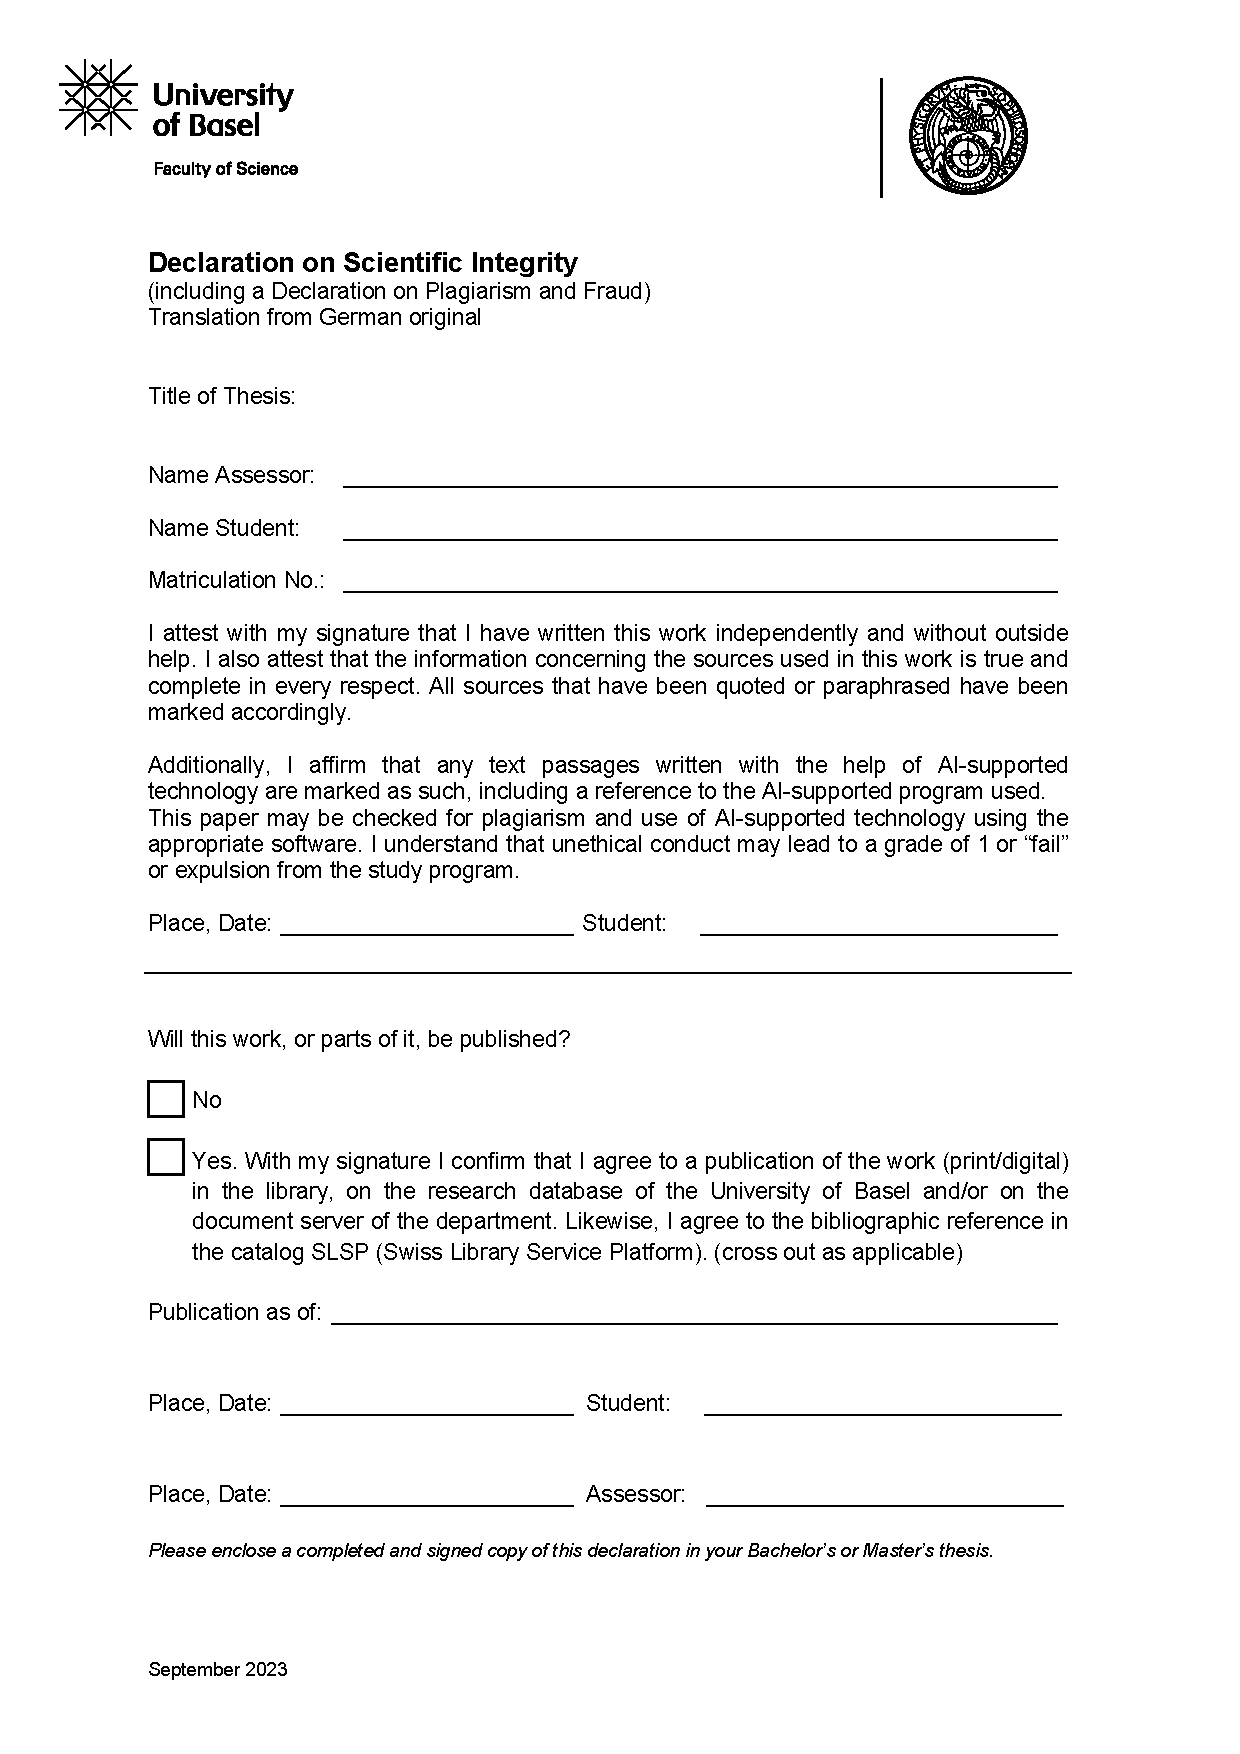
\includepdf{./Back/wissensch_Redlichkeit_E_09-2023.pdf}} %Maybe not needed ? 
  {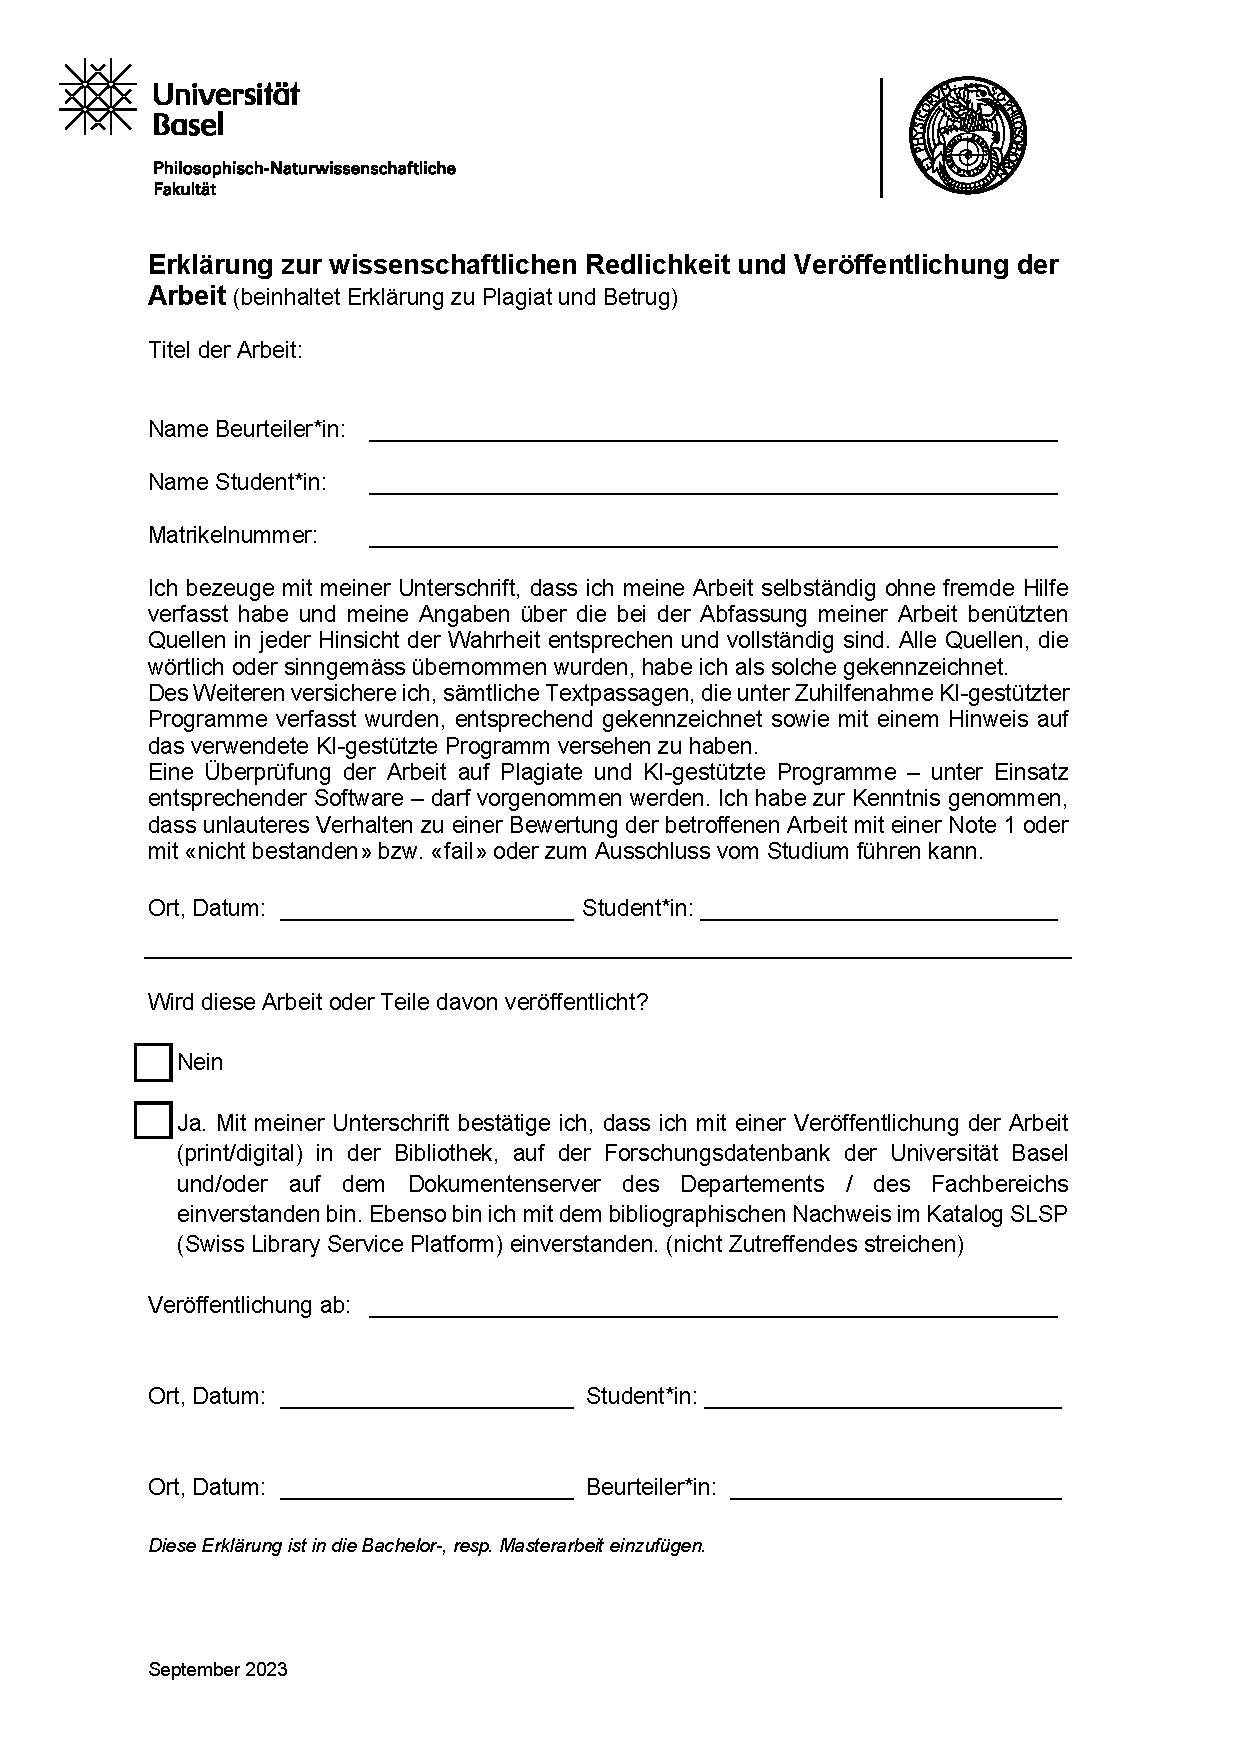
\includepdf{./Back/wissensch_Redlichkeit_D_09-2023.pdf}}
%% ----------------------------------------------------------------
\end{document}
%% ----------------------------------------------------------------
